\section{New Beam Screen Designs}

Using the knowledge acquired from examining the beam coupling impedance dependence on the layout of the beam screen from the previous section, and additionally the electrical field simulations of the induced voltages on the screen conductors during magnet pulsing, a number of alternative beam screen designs have been proposed. The motivation in these designs has been to reduce the power loss into the MKI (in this case to reduce the temperatures reached by the ferrite yoke) and to reduce the surface electric field of the ceramic tube, by the end of the screen conductors during magnet pulsing, to further reduce surface flashover between the screen conductors and along the ceramic tube to a ground plane.

The proposed designs are described below:

\begin{itemize}
\item{24 screen conductors of alternating length, as shown in Fig.~\ref{fig:24-alternating-length}. The alternating length screen conductors layout has been demonstrated to reduce the surface electric field associated with the shorter length screen conductors, thus being beneficial to the electrical breakdown rate of the shorter conductors. However the electric field associated with the longer screen conductors is increased.}
\item{24 screen conductors tapered in length, as shown in Fig.~\ref{fig:24-tapered-length}. The tapering of the screen conductors has previously been shown to help reduce the surface electric field of the shorter conductors in designs with 15 screen conductors.}
\item{24 screen conductors some with an alternating length and then tapered towards the HV busbar, as shown in Fig.~\ref{fig:24-alternating-tapered}. This mixture of the above two designs is intended to use the reduction of surface electric field of the shorter conductors due to the tapering, whilst keeping a relatively high capacitance at the capacitively coupled end so as to not induce additional worse resonances here or increase the beam coupling impedance of frequencies below 50MHz. Note that the alternating length screen conductors are closest to the return busbar and hence have the lowest induced voltage: hence an increase in the electric field of the longer conductors is not so important an effect.}
\item{24 screen conductors in enclosed slots in the ceramic tube, as shown in Fig.~\ref{fig:24-enclosed-slots}. The intention of this design is to increase the necessary induced voltage on the screen conductors before breakdown occurs, because surface flashover is no longer a possile breakdown path. This possible solution is discounted because of extreme difficulties associated with the manufacture of the ceramic tube \cite{Barnes:8thStratMeet}.}
\item{An alternative screen conductor layout, in which two conductors are conductively connected to ground at one end and all others are capacitively coupled to ground at both ends \cite{Barnes:mkiAlt}, as shown in Fig.~\ref{fig:alt-screen-design}. This design is intended to reduce the maximum induced voltage on the screen conductors by having all the screen conductors be connected to one another at the capacitively coupled end and being referenced to a voltage level approximately mid-way between the minimum and maximum induced voltage. To counter possible longitudinal eddy currents during pulsing reducing the field rise time, the majority of the screen conductors are capacitively coupled at both ends of the magnet, with two conductors connected to ground at the downstream end of the magnet.}
\item{24 alternating length screen conductors with part of the metallization replaced by a external metal cylinder, as shown in Fig.~\ref{fig:24-step-out-slight}. This design is intended to reduce the electric field at the capacitively coupled end by replacing the metallization on the external surface of the ceramic tube close to the ends of the screen conductors, with a metal cylinder some millimetres off the ceramic tube outer surface. Electric field simulations had shown that the high permittivity of the ceramic was in effect pushing the ground plane into the ceramic tube, reducing the effective spacing between the screen conductors and the metallization, whereas this physical air gap should reduce this effect \cite{Barnes:mkiAlt}.}
\item{24 screen conductors of a mixture of alternating and tapered lengths with part of the metallization replaced with an external metal cylinder \cite{Barnes:mkiElecSurfCer}, as shown in Fig.~\ref{fig:24-final-design}: the cylinder is 1mm from the outside surface of the ceramic tube at the return busbar side, and 3mm from the outisde surface of the ceramic tube at the HV busbar side. This was intended to improve on the above design by using the combined alternating and tapered design to further reduce the electric field on the surface of the ceramic tube associated with the screen conductors. Due to difficulty of manufacturing the step out of the metal cylinder is continued to the end of the ceramic tube. \textbf{This is the proposed final design for implementation in the replacement MKIs for installation during long shutdown 1 (2013-2014)}.}
\end{itemize}

\begin{figure}
\begin{center}
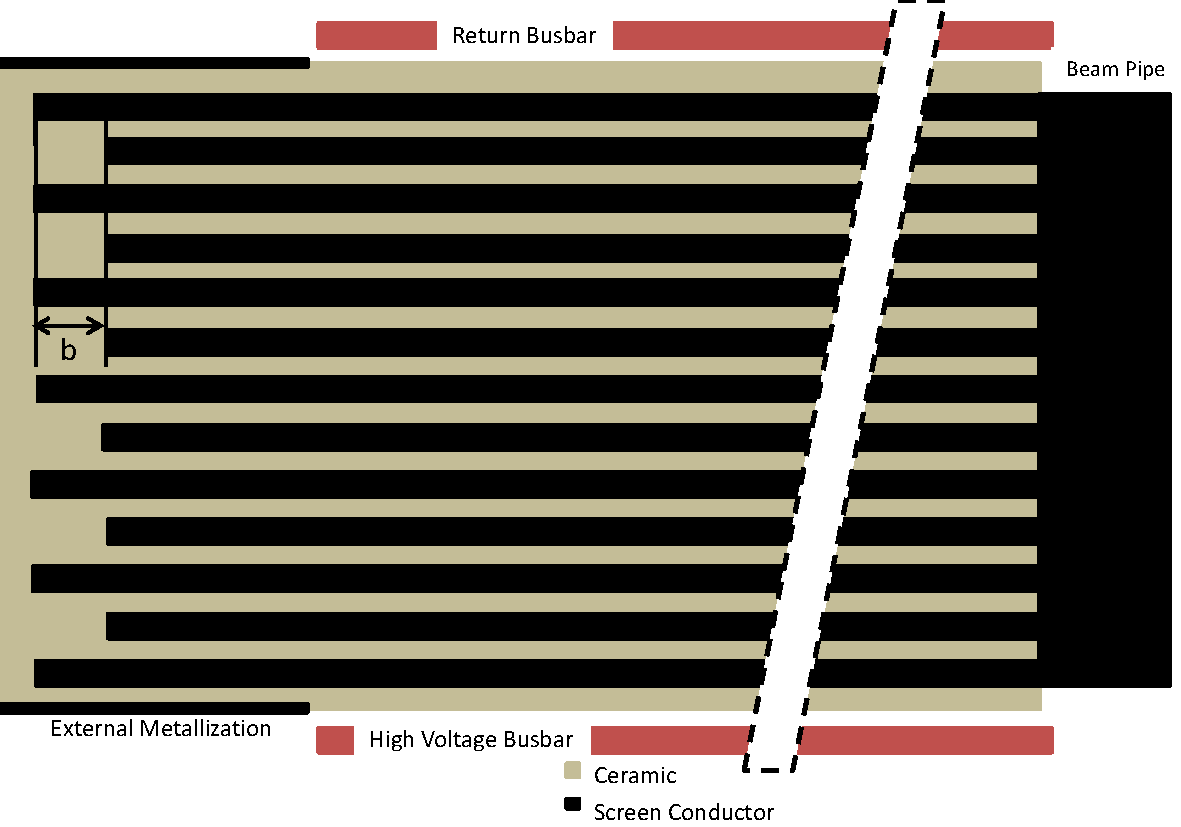
\includegraphics[width=0.7\textwidth]{LHC_MKI/figures/mki-design-layouts/alternating_screen_conductors.pdf}
\end{center}
\caption{A MKI beam screen design with alternating lengths of screen conductors - with a difference in length b.}
\label{fig:24-alternating-length}
\end{figure}
\begin{figure}
\begin{center}
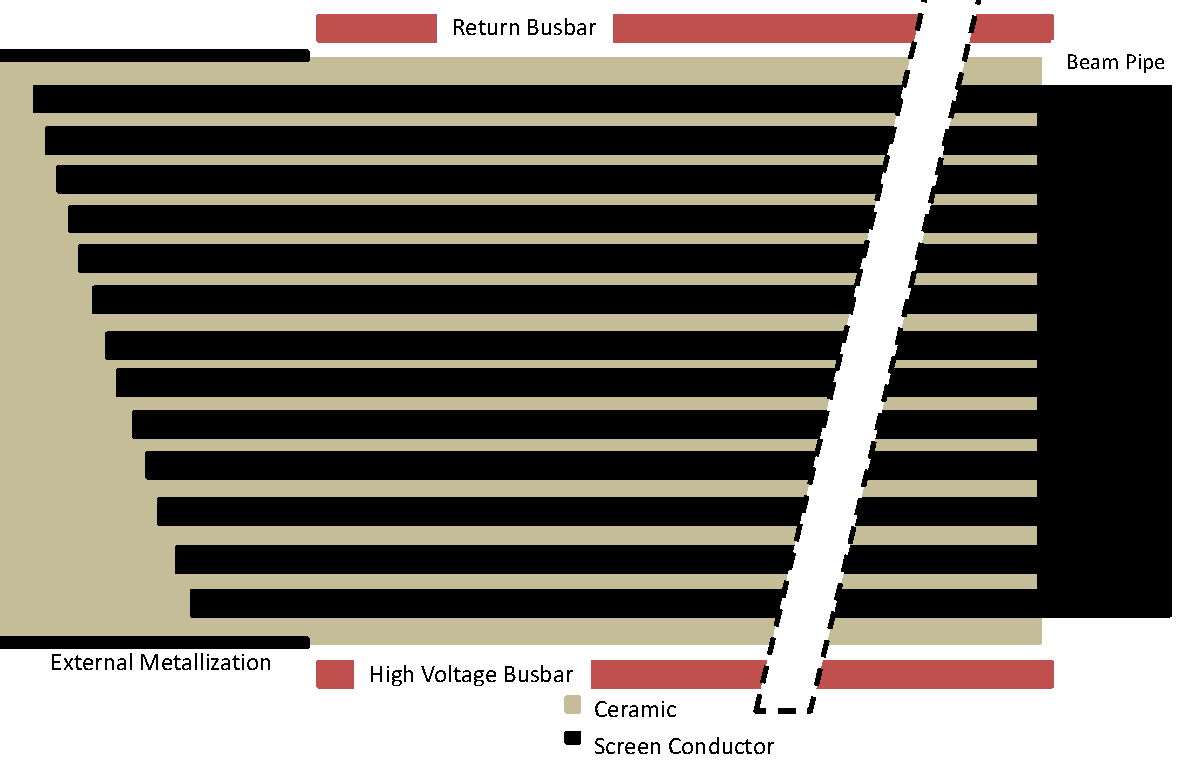
\includegraphics[width=0.7\textwidth]{LHC_MKI/figures/mki-design-layouts/shortening_screen_conductors.pdf}
\end{center}
\caption{A MKI beam screen design with tapered lengths of screen conductors. The taper may be altered to acquire the desired combination of impedance and surface electric field on the ceramic tube.}
\label{fig:24-tapered-length}
\end{figure}
\begin{figure}
\begin{center}
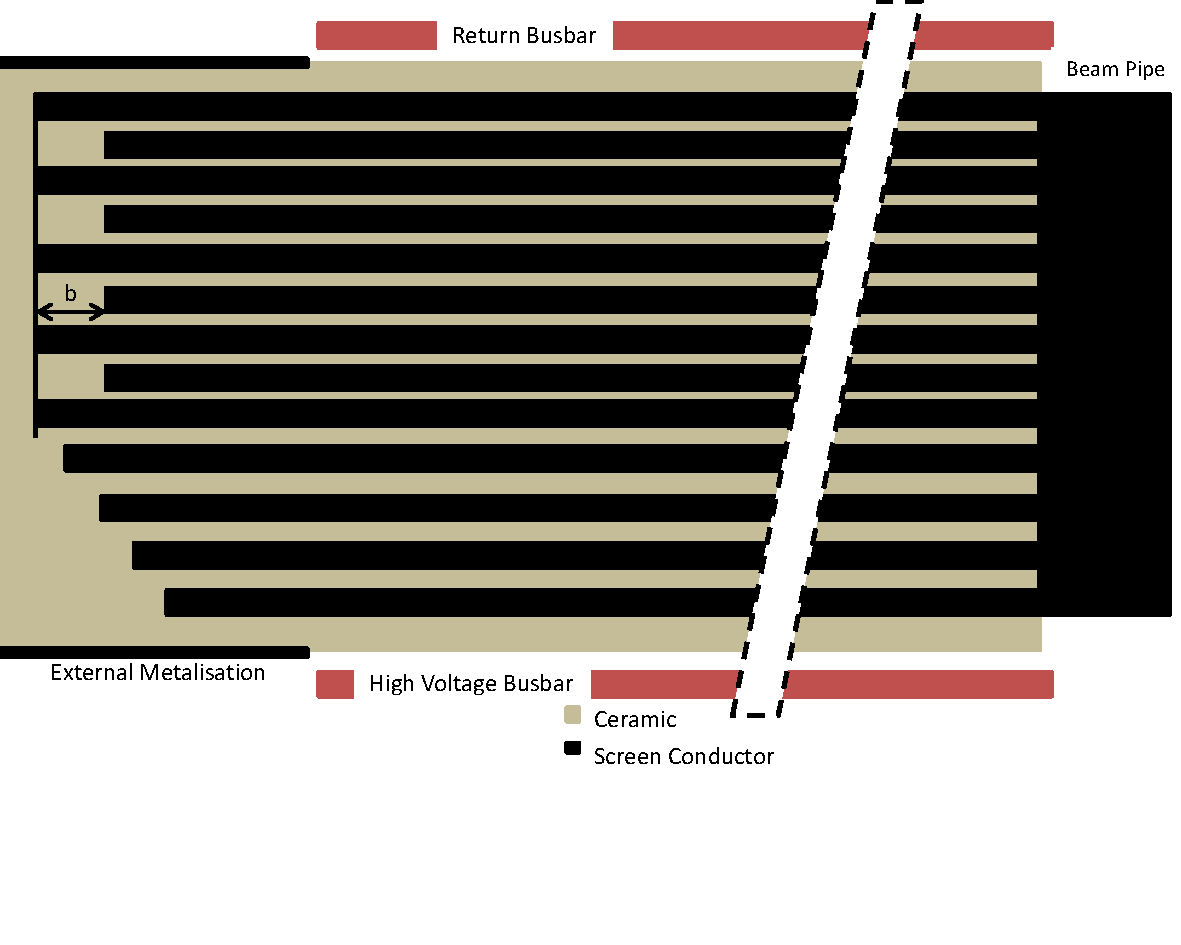
\includegraphics[width=0.7\textwidth]{LHC_MKI/figures/mki-design-layouts/combination_layout.pdf}
\end{center}
\caption{A MKI beam screen design with a combination of tapered and alternating screen conductors. The degree of alternating and tapering may change dependent of the desired impedance and surface electric field associated with the screen conductors. The alternating length conductors are closest to the return busbar.}
\label{fig:24-alternating-tapered}
\end{figure}

\begin{figure}
\begin{center}
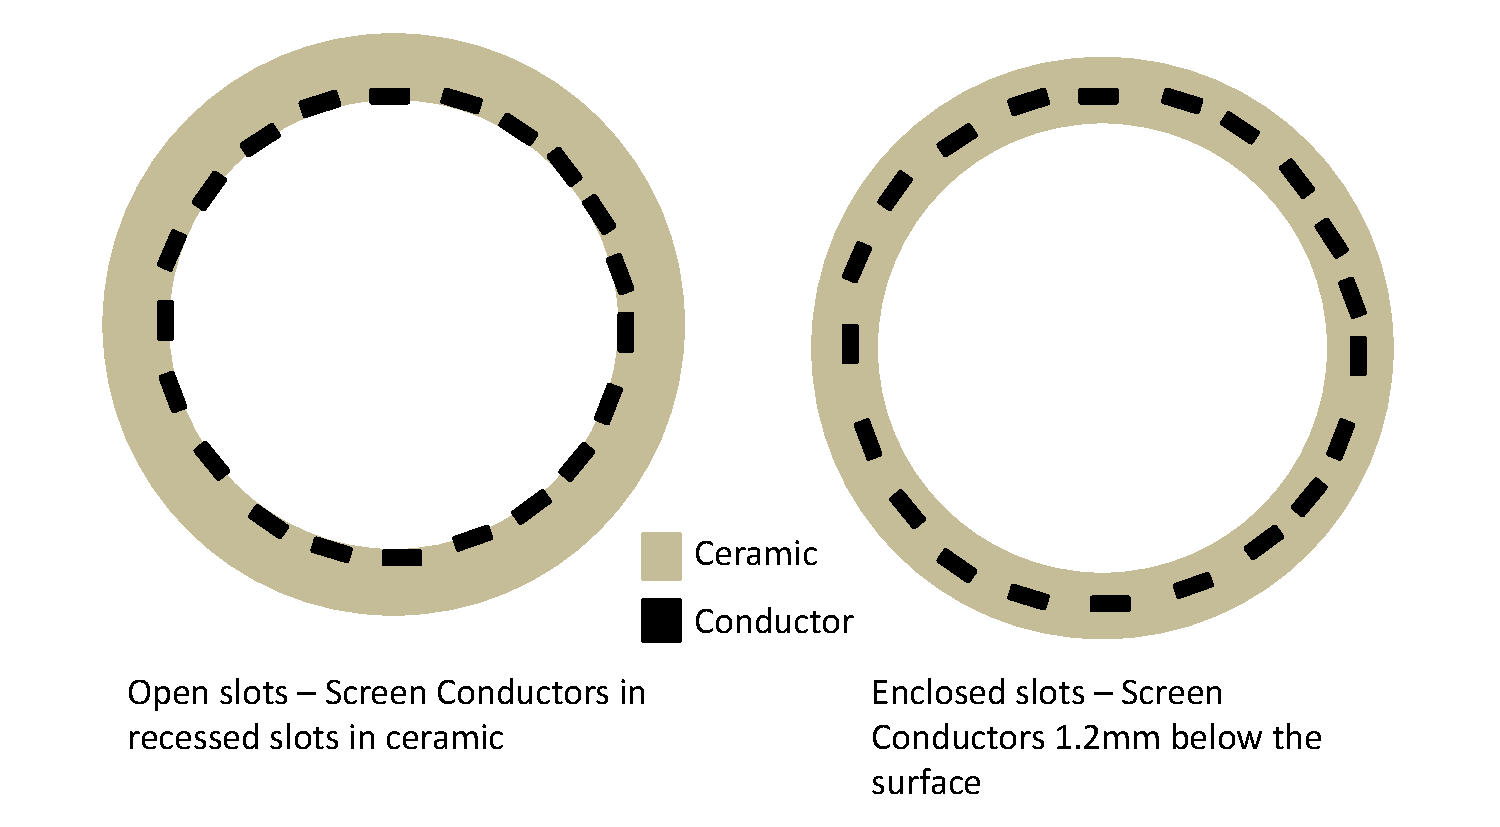
\includegraphics[width=0.7\textwidth]{LHC_MKI/figures/mki-design-layouts/enclosed_diagram.pdf}
\end{center}
\caption{A MKI beam screen design with enclosed slots (shown in comparison to the usual beam screen design with open slots) for the screen conductors.}
\label{fig:24-enclosed-slots}
\end{figure}

\begin{figure}
\begin{center}
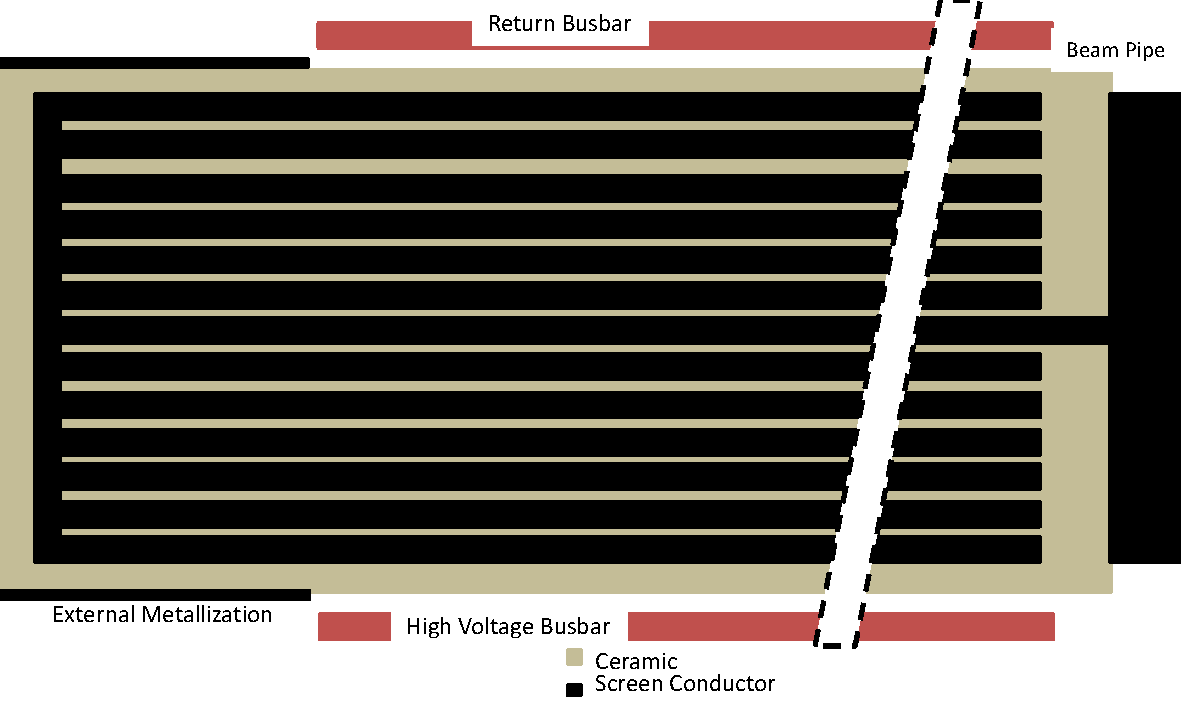
\includegraphics[width=0.7\textwidth]{LHC_MKI/figures/mki-design-layouts/alternative_screen_design.pdf}
\end{center}
\caption{A MKI beam screen design using an alternative screen conductor layout in which 2 (cross section shown here) conductors are connected to ground at one end of the screen, and all conductors are connected together at the other end. Both ends have capacitive coupling.}
\label{fig:alt-screen-design}
\end{figure}

\begin{figure}
\begin{center}
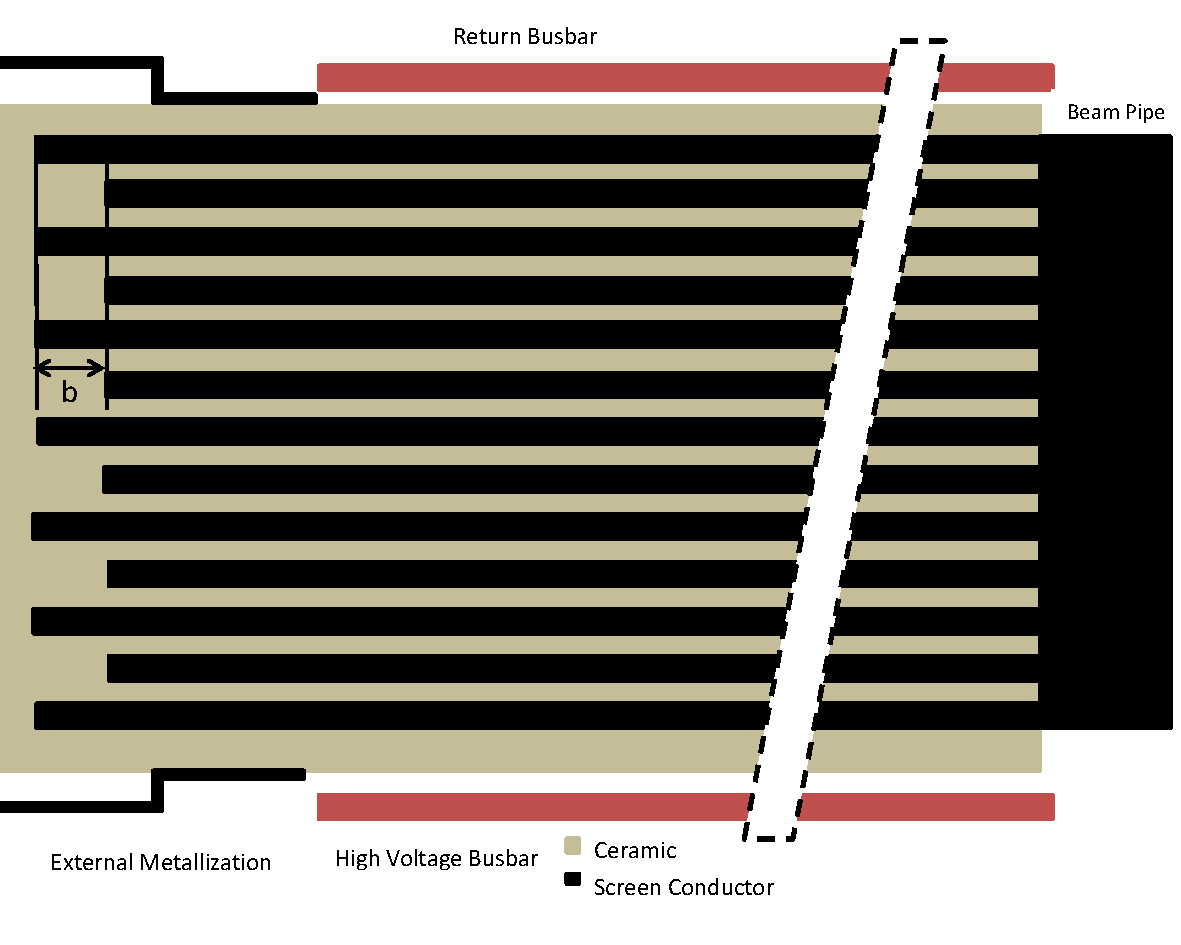
\includegraphics[width=0.7\textwidth]{LHC_MKI/figures/mki-design-layouts/alternating_screen_conductors_step_out_metallisation.pdf}
\end{center}
\caption{A MKI beam screen design implementing a replacement of some of the external metallization with a metallic cylinder so as to remove the ground plane closest to the ends of the screen conductors from the outer surface of the ceramic tube.}
\label{fig:24-step-out-slight}
\end{figure}

\begin{figure}
\begin{center}
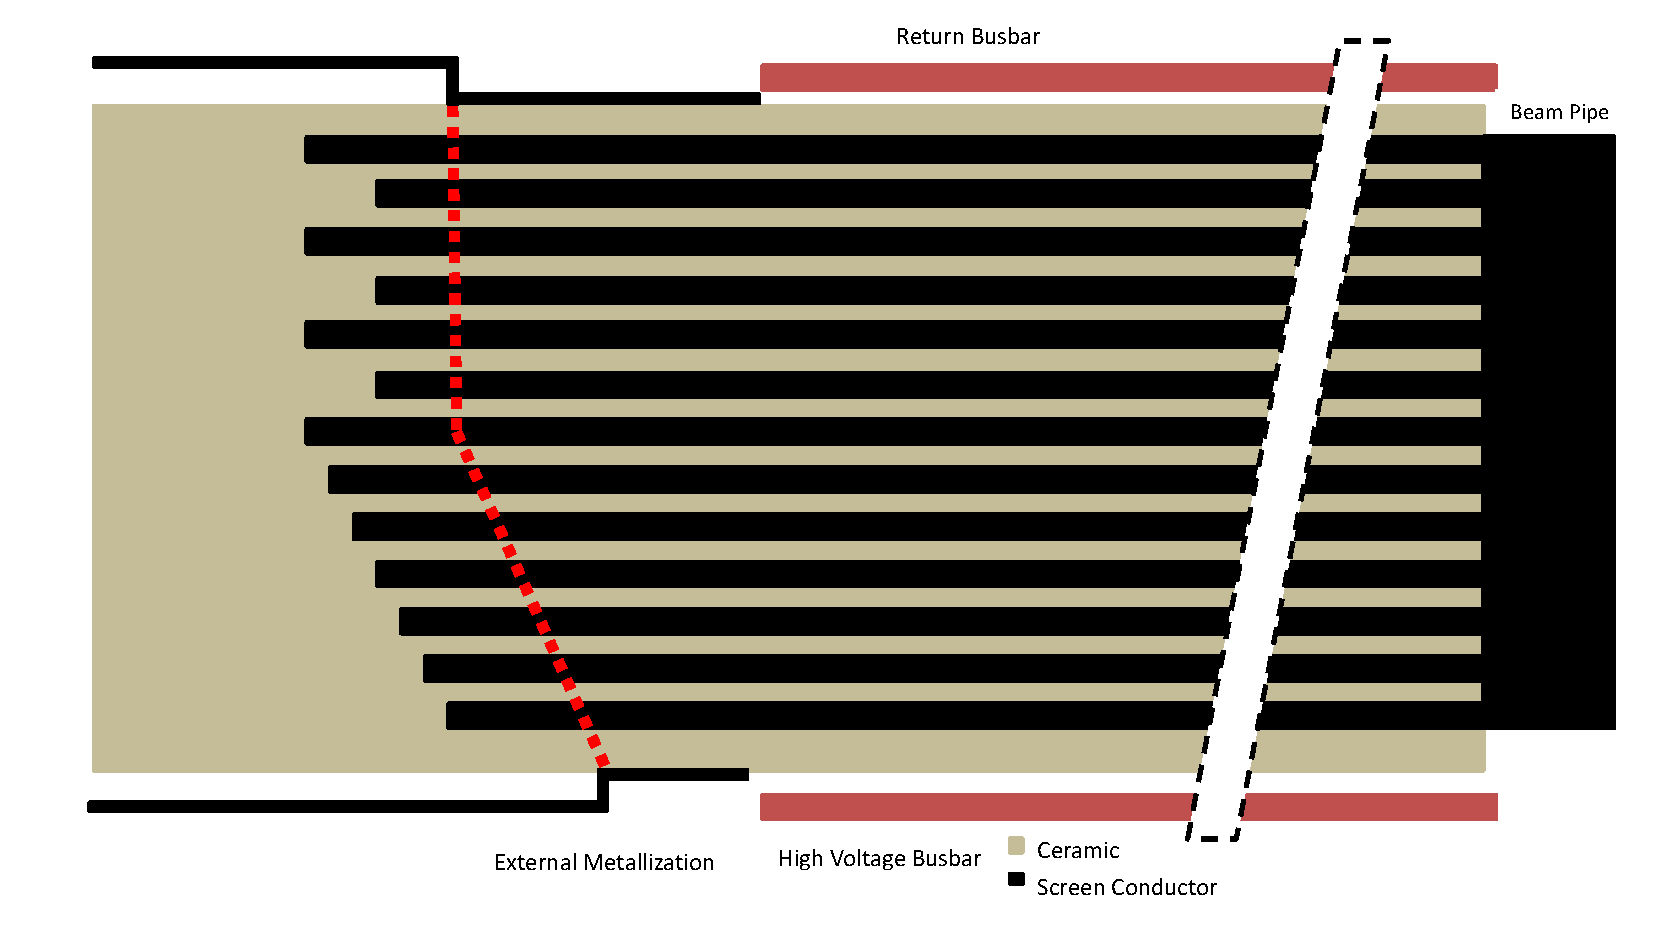
\includegraphics[width=0.7\textwidth]{LHC_MKI/figures/mki-design-layouts/mki-final-design.pdf}
\end{center}
\caption{The proposed final MKI design. A combination of alternating and tapered screen conductors is used, along with a step out of the external metallization to a metal cylinder. The outline of the step out is shown by the red-dashed line.}
\label{fig:24-final-design}
\end{figure}

In this analysis of these designs we shall focus on the resulting power loss from interaction of the beam with the real component of the longitudinal beam impedance as this is the present primary limitation from the MKIs. The real component of the longitudinal beam coupling impedance is shown in Fig.~\ref{fig:new-screen-designs-mki}, and the imaginary in Fig.~\ref{fig:new-screen-designs-mki-imag}.

\begin{figure}
\begin{center}
\subfigure[]{
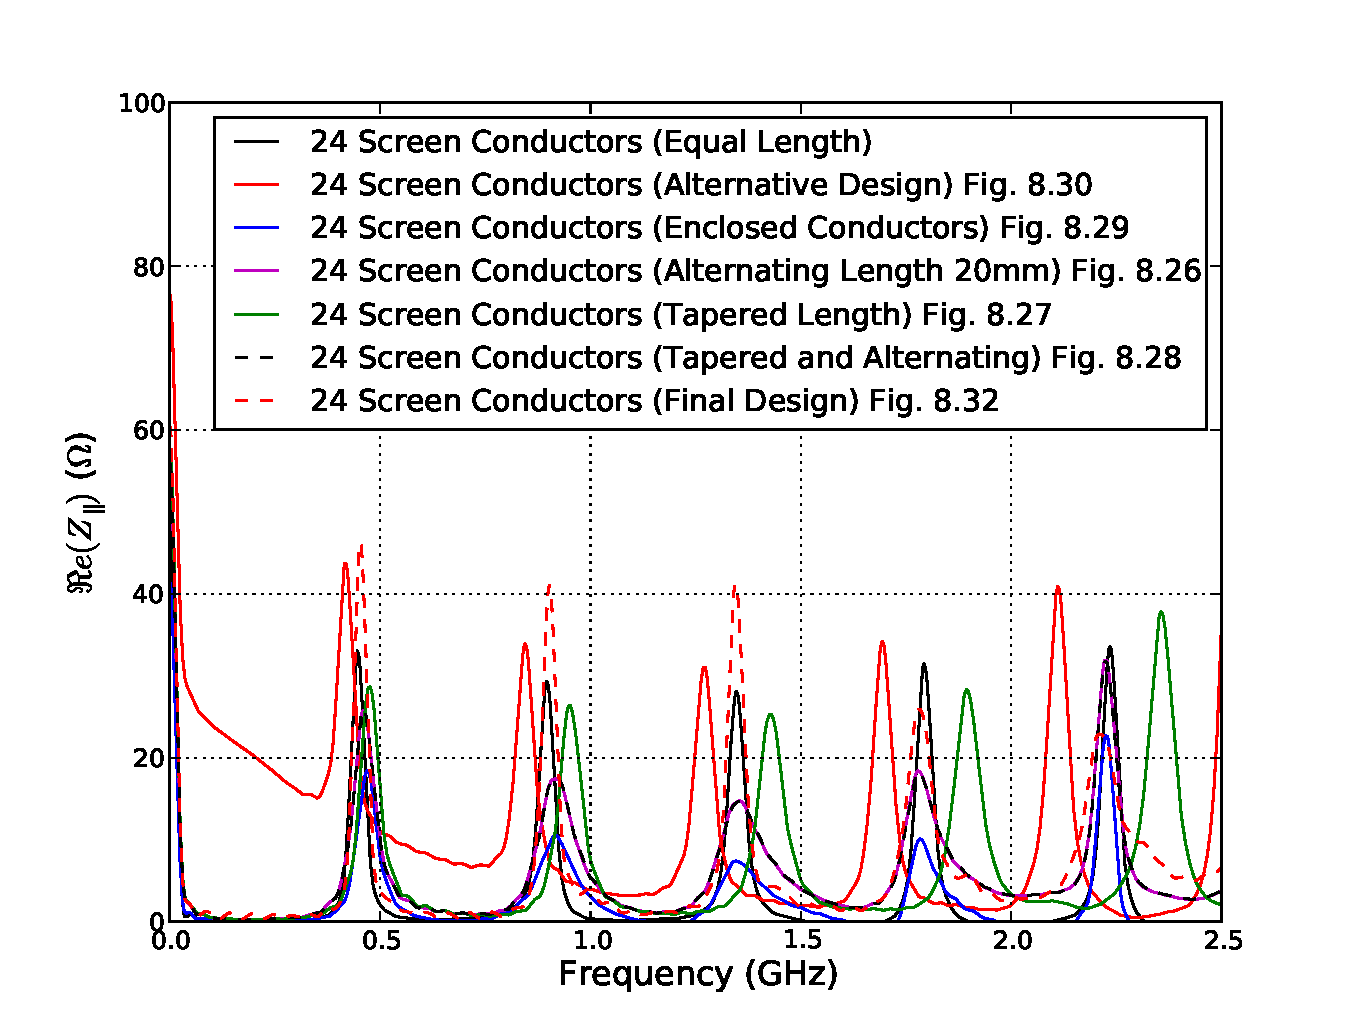
\includegraphics[width=0.85\textwidth]{LHC_MKI/figures/mki-new-screen-designs-impedance-real.pdf}
\label{fig:new-screen-designs-mki}
}
\subfigure[]{
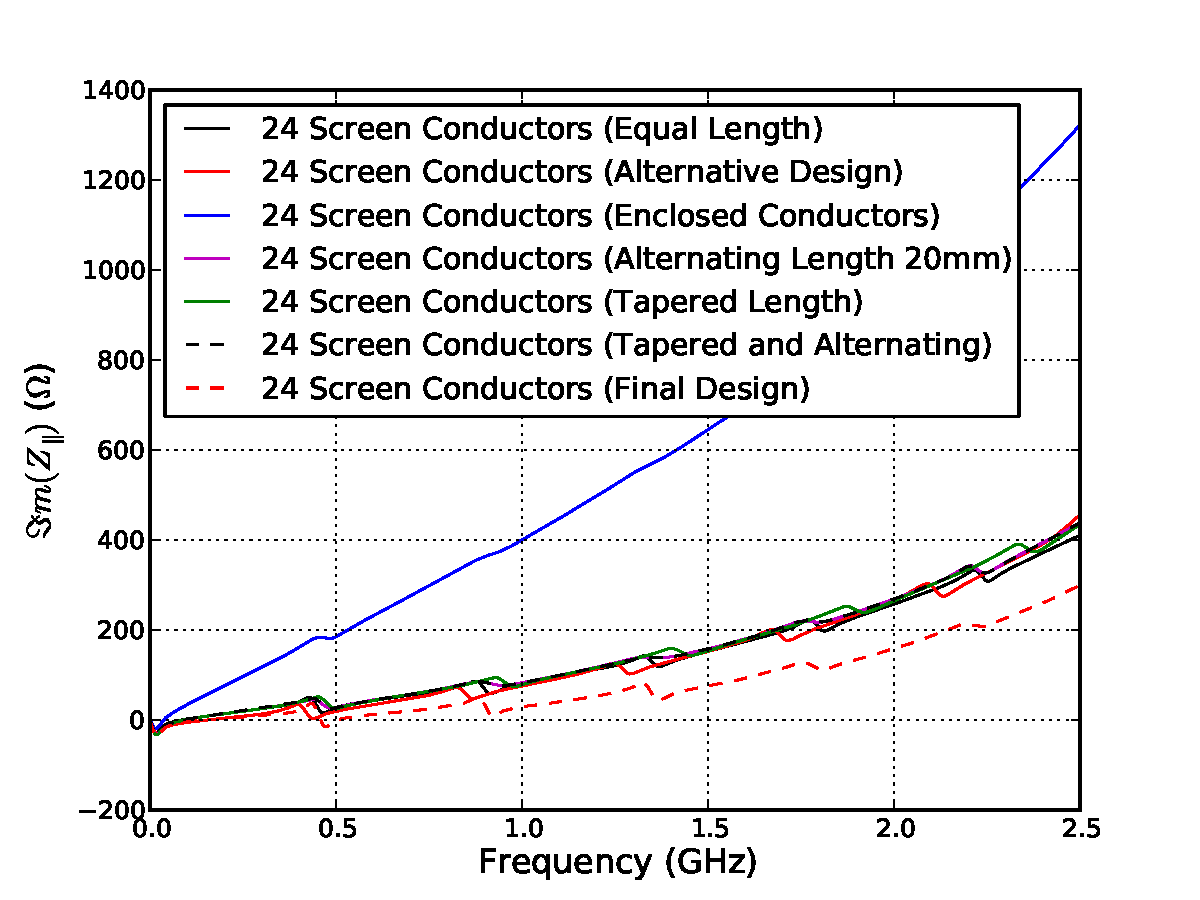
\includegraphics[width=0.85\textwidth]{LHC_MKI/figures/mki-new-screen-designs-impedance-imag.pdf}
\label{fig:new-screen-designs-mki-imag}
}
\end{center}
\caption{The real component of the beam coupling impedance for a number of the proposed beam screen designs \ref{fig:new-screen-designs-mki}. In addition the imaginary component of the longitudinal impedance is shown for completeness \ref{fig:new-screen-designs-mki-imag}. In all cases the outside diameter of the ceramic tube is 56mm.}
\end{figure}

The estimated heating for both 25ns and 50ns bunch spacing operation in the LHC are shown in Tab.~\ref{tab:heating-mki-screen-designs} for 1ns bunch length, and the variation in power loss with the bunch length for 25ns and 50ns bunch spacing shown in Fig.~\ref{fig:mki-screens-heating-bunch-length}. It can be seen that the power loss can be very strongly reduced for very short bunch lengths (as has been proposed for HL-LHC operation without crab cavities \cite{Bruning:beamParameters}) by increasing the bunch length, but for nominal bunch lengths ($\tau_{b}=$1ns) it can be seen that there is not much benefit in further increasing the bunch length.

\begin{table}
\caption{The power loss expected due to beam-wakefield interactions in the MKIs for a number of proposed beam screen designs. Estimates are given for 50ns and 25ns bunch spacing in the LHC (1380 bunches, $1.7 \times 10^{11}$ particles per bunch for 50ns, 2808 bunches, $1.15 \times 10^{11}$ particles per bunch for 25ns) assuming a cos$^{2}$ bunch distribution.}
\label{tab:heating-mki-screen-designs}
\begin{center}
\begin{tabular}{c | c | c}
Screen Design & $P_{loss,50ns}$ (W), $t_{b}=1$ns & $P_{loss,25ns}$ (W), $t_{b}=1$ns \\ \hline 
24 Conductors, Alternating Length & 36 & 28 \\ \hline %full length
24 Conductors, Tapered Length & 36 & 27 \\ \hline %full length
24 Conductors, Alternating and Tapered & 36 & 28 \\ \hline %full length
24 Screen Conductors, Enclosed Conductors & 21 & 17 \\ \hline %full length
24 Conductors, Alternate Design & 182 & 161 \\ \hline %full length
24 Conductors, Step out & 37 & 30 \\ \hline %Shortened
24 Conductors, Final Design & 37 & 30 \\ %full length
\end{tabular}
\end{center}
\end{table}

\begin{figure}
\subfigure[]{
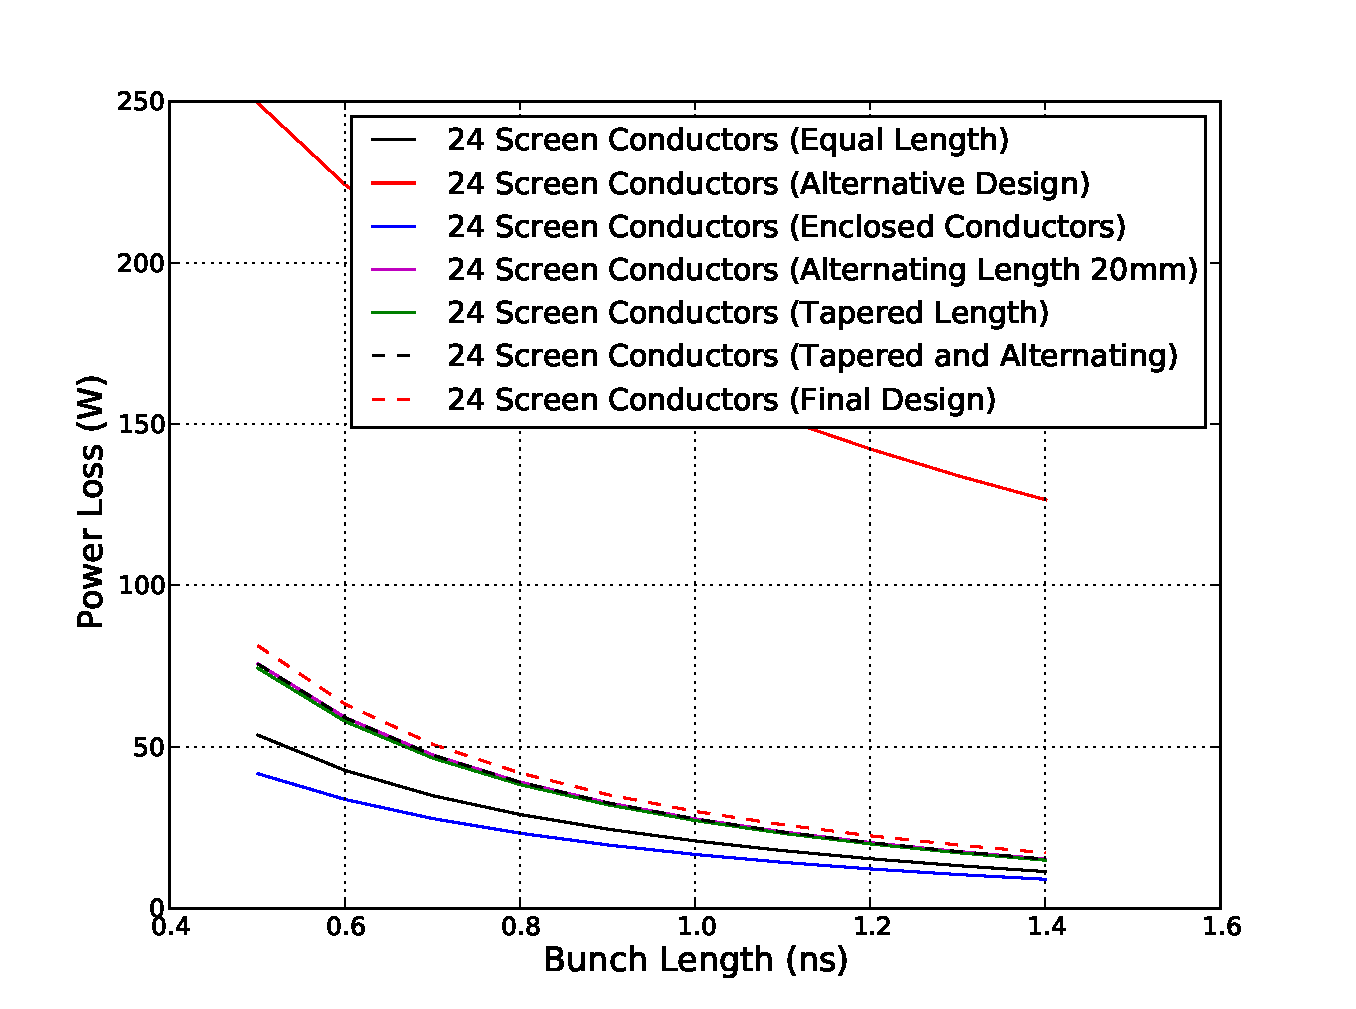
\includegraphics[width=0.5\textwidth]{LHC_MKI/figures/mki-new-designs-heating-25ns.pdf}
\label{fig:mki-screen-heating-25ns}
}
\subfigure[]{
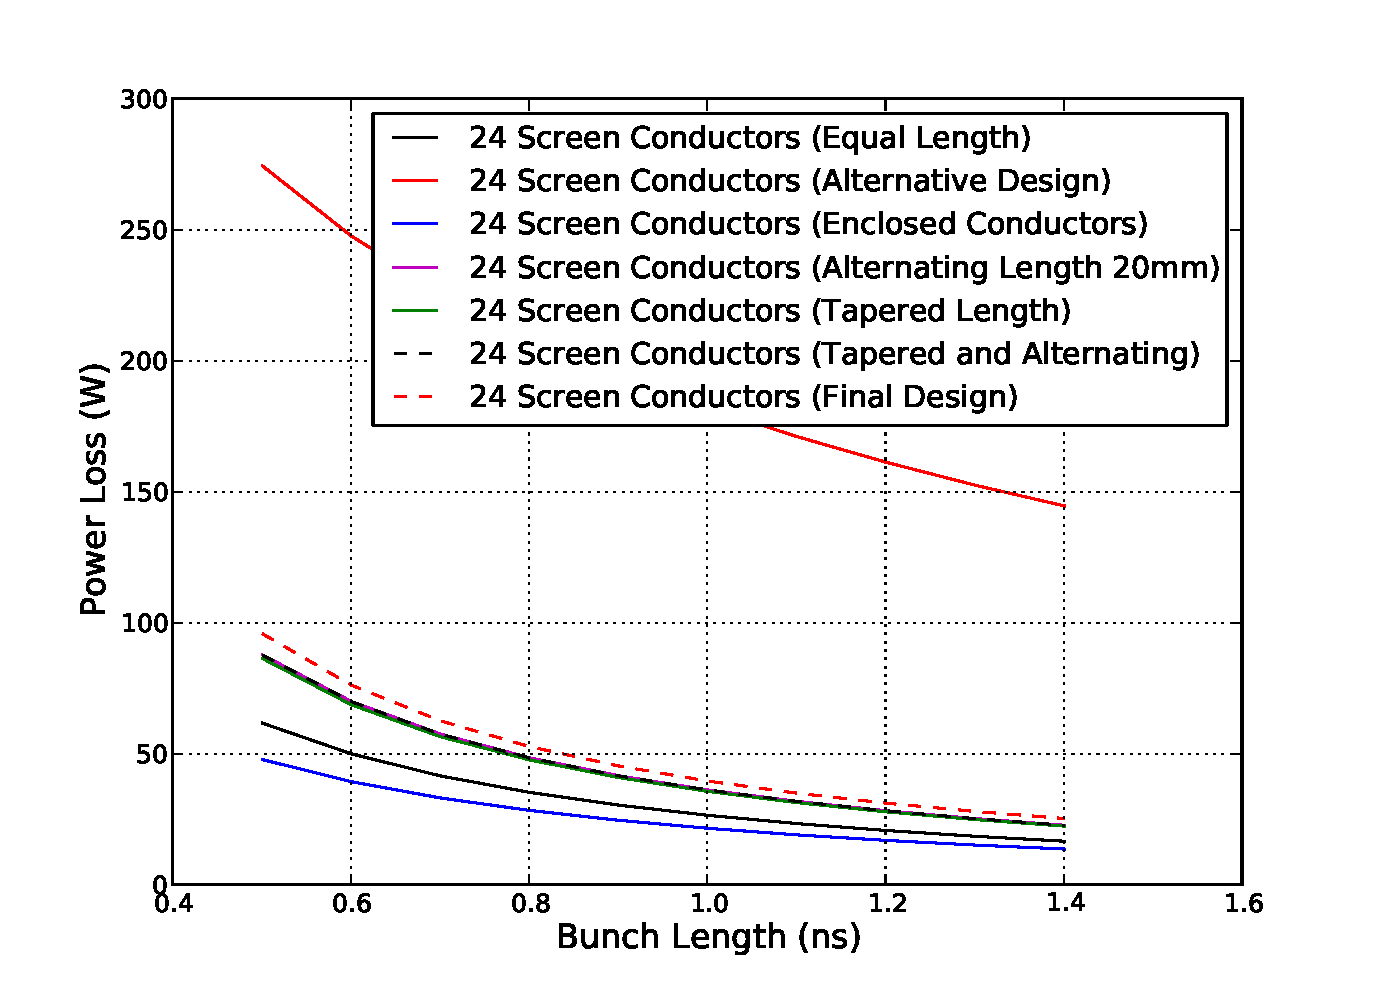
\includegraphics[width=0.5\textwidth]{LHC_MKI/figures/mki-new-designs-heating-50ns.pdf}
\label{fig:mki-screen-heating-50ns}
}
\caption{The variation of the predicted beam induced power loss with bunch length for a number of screen designs. The variation for 25ns \ref{fig:mki-screen-heating-25ns} and 50ns \ref{fig:mki-screen-heating-50ns} machine settings.}
\label{fig:mki-screens-heating-bunch-length}
\end{figure}
